% Currently unused

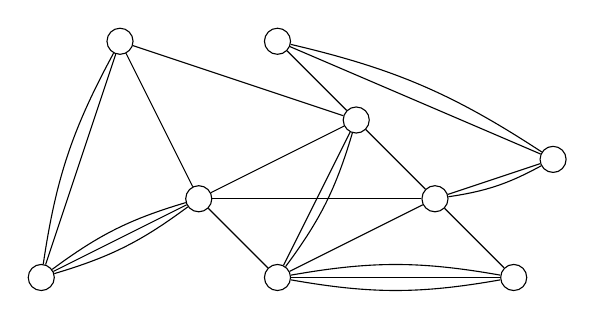
\begin{tikzpicture}
  \begin{scope}[every node/.style={circle, draw}]
    \node (a) at (0,0) {} ;
    \node (b) at (-1,2) {} ;
    \node (c) at (1,-1) {} ;
    \node (d) at (2,1) {} ;
    \node (e) at (1,2) {} ;
    \node (f) at (-2,-1) {} ;
    \node (g) at (3,0) {} ;
    \node (h) at (4,-1) {} ;
    \node (i) at (4.5,0.5) {} ;
  \end{scope}

  \begin{scope}[-]
    \draw (a) to (b);
    \draw (a) to (c);
    \draw (a) to (f);
    \draw (a) to (d);
    \draw (a) to (g);
    \draw (b) to (f);
    \draw (c) to (h);
    \draw (c) to (g);
    \draw (d) to (c);
    \draw (d) to (b);
    \draw (g) to (h);
    \draw (g) to (i);
    \draw (g) to (d);
    \draw (e) to (d);
    \draw (e) to (i);
    % \draw (e) to (a);
    \draw (f) to[bend left=10] (b);
    \draw (f) to[bend left=10] (a);
    \draw (f) to[bend right=10] (a);
    \draw (e) to[bend left=10] (i);
    \draw (g) to[bend right=10] (i);
    \draw (c) to[bend right=10] (d);
    \draw (c) to[bend right=10] (h);
    \draw (c) to[bend left=10] (h);
  \end{scope}
\end{tikzpicture}


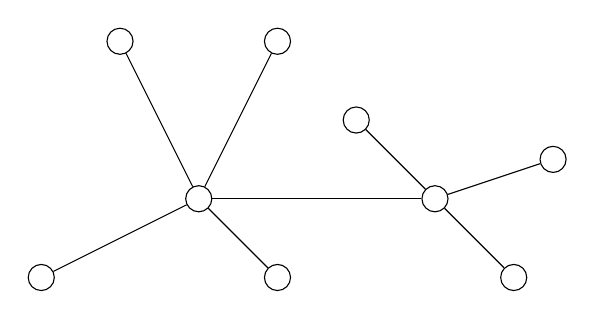
\begin{tikzpicture}
  \begin{scope}[every node/.style={circle, draw}]
    \node (a) at (0,0) {} ;
    \node (b) at (-1,2) {} ;
    \node (c) at (1,-1) {} ;
    \node (d) at (2,1) {} ;
    \node (e) at (1,2) {} ;
    \node (f) at (-2,-1) {} ;
    \node (g) at (3,0) {} ;
    \node (h) at (4,-1) {} ;
    \node (i) at (4.5,0.5) {} ;
  \end{scope}

  \begin{scope}[-]
    \draw (a) to (b);
    \draw (a) to (c);
    \draw (a) to (f);
    \draw (a) to (e);
    \draw (a) to (g);
    \draw (g) to (h);
    \draw (g) to (i);
    \draw (g) to (d);
  \end{scope}
\end{tikzpicture}
